\documentclass[10pt]{beamer}

\mode<presentation> 
{ \usetheme[nat,dogma]{Frederiksberg} }

% \usepackage[danish]{babel}
\usepackage[latin1]{inputenc}
\usepackage{times}
\usepackage[T1]{fontenc}
\usepackage[english]{babel}
\usepackage{hyperref}
\usepackage{animate}
%\usepackage{multimedia}
\usepackage{francois-preamble}
\usepackage{multirow}

\usepackage{multirow}
%\usepackage{movie15}

\newcommand{\cc}{{c\!\!,}}
\newcommand{\degr}[1]{{{#1}^\circ}}


\title{Vision and Image Processing:\\ Disparity, Stereo Matching}

\author[F.~Lauze] % (optional, use only with lots of authors)
{Fran{\c c}ois Lauze}

\institute[DIKU] % (optional, but mostly needed)
{
  Department of Computer Science\\
  University of Copenhagen
}

\date[2013-2014 B2] % (optional, should be abbreviation of conference name)
% {Research Presentation, Diku 2006}

\definecolor{gold}{rgb}{0.95,0.83,0.0}
\definecolor{orange}{rgb}{0.95,0.7,0.0}
% \definecolor{backblue}{rgb}{0.93,0.94,0.99}
\definecolor{backblue}{rgb}{0.95,0.94,0.99}
\setbeamercolor*{background canvas}{bg=backblue} 



\newcommand{\myemph}[1]{{\color{blue}{#1}}}
\newcommand{\intrg}[1]{\int_{{#1}=-\infty}^\infty}
\newcommand{\intRR}{\int_{-\infty}^\infty}

\AtBeginSection[]
{
  \begin{frame}<beamer>{Outline}
    \tableofcontents[currentsection,currentsubsection]
  \end{frame}
}

\begin{document}
\maketitle

% would be cool with more images showing applications


%-------------------------------------------------------------------
%   Start slides
%-------------------------------------------------------------------




%----------------------------------------------



\begin{frame}
  \frametitle{Topics for today's lecture}
  \begin{itemize}
  \item Binocular Disparity
  \item Depth and Disparity
  \item Stereo Matching
  \item Dense Matching vs. Optical Flow
  \end{itemize}
\end{frame}



\begin{frame}
  \frametitle{Binocular Disparity\footnote{Pictures from Wikipedia.}}
  \begin{center}
    \begin{tabular}[h]{cc}
       \includegraphics[width=0.3\textwidth]{FIGURES/Binocular_disparity1}&
       \includegraphics[width=0.3\textwidth]{FIGURES/Binocular_disparity2}\\
       Binocular Disparity & Disparity simulation.
    \end{tabular}
  \end{center}
\end{frame}



\begin{frame}
  \frametitle{Binocular Disparity I}
  \begin{columns}
    \column{0.4\textwidth}
    \begin{center}
       \includegraphics[width=0.9\textwidth]{FIGURES/Binocular_disparity1}
    \end{center}
    \column{0.6\textwidth}
    \begin{itemize}
    \item Black dot: fixation point.
    \item Green dot: point with far disparity.
     Angle with direction of fixation point is small.
    \item Blue dot: point with near disparity.
      Angle with direction of fixation point is large.
    \end{itemize}
  \end{columns}
\end{frame}




\begin{frame}
  \frametitle{Binocular Disparity II} 
  \begin{columns}
    \column{0.4\textwidth}
    \begin{center}
       \includegraphics[width=0.9\textwidth]{FIGURES/Binocular_disparity2}
    \end{center}
    \column{0.6\textwidth}
    \begin{itemize}
    \item Object at depth $\not=$ fixation depth.
    \item Can be simulated by presenting laterally shifted image to
      the other eye.
    \item Principle behind 3D movies.
    \item Some explanations to follow!
    \end{itemize}
  \end{columns}
\end{frame}



\begin{frame}
  \frametitle{A Reminder from Last Week I} 
  \begin{center}
    \includegraphics[width=0.9\textwidth]{FIGURES/stereo}
  \end{center}
  If we can recover $x'$ from $x$ we can recover depth.
\end{frame}

\begin{frame}
  \frametitle{Reminder II}
  \begin{center}
    \includegraphics[width=0.9\textwidth]{FIGURES/epigeom}
  \end{center}
  \begin{itemize}
  \item Line connecting $O$ and $O'$: \myemph{baseline}
  \item Plane through baseline $x$ and $x'$: \myemph{Epipolar Plane}
  \item \myemph{Epipoles}: intersection of baseline and image planes:
    projection of the other camera center.
  \item \myemph{Epipolar Lines} - intersections of epipolar plane with image
    planes (always come in corresponding pairs)
  \end{itemize}  
\end{frame}


\begin{frame}
  \frametitle{How: Parallel Case}
  \begin{columns}
    \column{0.5\textwidth}
    \includegraphics<1-2>[width=1\textwidth]{FIGURES/stereoparallel}
    \includegraphics<3->[width=1\textwidth]{FIGURES/stereoparallel2}
    \column{0.5\textwidth}
    {\small 
      Simple situation:
      \begin{itemize}
      \item Parallel image planes and parallel to baseline.
      \item Camera centers at same height
      \item same focal length.
      \end{itemize}
    }
    \pause
    {\small 
      For instance:
      \begin{itemize}
      \item Two pictures obtained from the same camera, translating
        along its $x$-axis.
      \end{itemize}
    }
    \pause
    {\small
      Implication:
      \begin{itemize}
      \item Epipolar lines are horizontal scan lines!
      \item Epipoles are at $\infty$.
      \end{itemize}
    }
  \end{columns}
\end{frame}


\begin{frame}
  \frametitle{Depth from Disparity}
  \underline{\href{http://en.wikipedia.org/wiki/Intercept_theorem}{Intercept Theorem again!}} 
  \begin{center}
    \includegraphics[width=0.75\textwidth]{FIGURES/dispdepth1d}
  \end{center}
  \begin{itemize}
  
  \item disparity := $x'-x = B -\overline{P_L P_R}$
  \end{itemize}
\end{frame}


\begin{frame}
  Apply Intercept Theorem to previous figure:
  $$
  \frac{\overline{P_L P_R}}{B} = \frac{z-f}{z}\quad \Iff \quad
  z\times \overline{P_L P_R} = B\times\left(z-f\right)
  $$
  $$
  \Updownarrow
  $$
  $$
  z\times\udesc{\text{disparity}}{\left(B-\overline{P_L P_R}\right)} = B\times f\quad
  \Iff\quad
  \text{disparity} = \frac{B\times f}{z}
  $$\vfill
  \pause
  \begin{block}{Depth and Disparity}
      Disparity is inversely proportional to depth.
  \end{block}
\end{frame}



\begin{frame}
  \frametitle{Computing Disparity: Simple Settings}
  \begin{itemize}
  \item Calibrated parallel cameras, with identical parameters.
  \item Search matches along scan lines, they are the epipolar lines
    of the 2-views problem.
  \item Extract disparity from Match positions.
  \end{itemize}
\end{frame}

\begin{frame}
  \frametitle{Example}
  \begin{center}
    \includegraphics<1>[width=\textwidth]{FIGURES/moensmand1}
    \includegraphics<2>[width=\textwidth]{FIGURES/moensmand2}
    \includegraphics<3>[width=\textwidth]{FIGURES/moensmand3}
    \includegraphics<4>[width=\textwidth]{FIGURES/moensmand4}\\
    Searching for match along scan lines.
  \end{center}
  \begin{itemize}
  \item Feature based Disparity maps:
  \item Search interest point matches along scan lines.
  \item Disparities computed only at these interest points:
  \item If more needed, interpolation or dense disparity maps?
  \end{itemize}

\end{frame}


\begin{frame}
  \frametitle{Non horizontal Scan lines}
  \begin{itemize}
  \item What when cameras are in more general position?, calibration is unknown?
  \item If calibration known, the essential matrix provides epipolar constraints.
  \item Non calibrated views: Estimate the fundamental matrix. 
  \item Knowing Essential or Fundamental matrix allows for image rectification.
  \item To know more on fundamental matrices: \underline{\href{http://danielwedge.com/fmatrix}{follow the link!}}
  \end{itemize}
\end{frame}


\begin{frame}
  \frametitle{Projective Rectification}
  \begin{columns}
    \column{0.6\textwidth}
    \includegraphics[width=\textwidth]{FIGURES/stereorect}
    \column{0.4\textwidth}
    \begin{itemize}
    \item Reproject onto a common plane parallel to line between camera centers
    \item Projections are homographies!
    \item Pixel motion is horizontal after reprojection.
    \item Cf Loop-Zhang, CVPR 1999.
    \end{itemize}
  \end{columns}
\end{frame}


\begin{frame}
  \frametitle{Projective Rectification example}
  \begin{center}
    \includegraphics[width=0.8\textwidth]{IMAGES/projrectexpl}
  \end{center}
\end{frame}




\begin{frame}
  \frametitle{Disparity Map}
  \begin{itemize}
  \item Still simple model: Horizontal scan lines.
  \item $d(x,y)$ = disparity of pixel at position $(x,y)$. Assume intensity conserved
    $$
    I_2(x+d(x,y),y) = I_1(x,y)
    $$
  \item Similar to Displaced Frame Difference in Optical Flow
    $$
    I_2(x+v_1(x,y), y+v_2(x,y)) = I_1(x,y)
    $$
  \item Displacement only along one direction: compared to Optical Flow, \myemph{no aperture problem!}
  \item This does not mean that computing disparity is easy...
  \end{itemize}
\end{frame}

\begin{frame}
  \frametitle{Differential Form}
  \begin{itemize}
  \item Mimic Optical Flow idea: linearize the disparity constraint
    \begin{align*}
      I_2(x+d(x,y),y) - I_1(x,y) &\approx \udesc{\tilde{I}_t}{I_2(x,y) - I_1(x,y)} + \pder{I_2}{x} d(x,y)\\
      &\approx 0
    \end{align*}
    \item At each pixel: 1 equation and 1 unknown: can be solved.
    \item Would give the solution
      $$
      d(x,y) = - \frac{\tilde{I_t}}{{I_{2x}}}
      $$
      \item Similar to 1D optical Flow.
    \item Above equation does not often hold because of: Noise in measurement, flat regions, shadows, repetitions... 
    \end{itemize}
\end{frame}

\begin{frame}
  \begin{center}
    \includegraphics[width=\textwidth]{IMAGES/ddmapbad}
  \end{center}
\end{frame}



\begin{frame}
  \frametitle{Regularization of the problem}
  \begin{itemize}
  \item Assume generally slowly varying disparity map, solve in least-squares sense.\vfill
  \item Many possibilities: \vfill
    \begin{itemize}
    \item Block Matching approach.\vfill
    \item Adaptation of the Lucas-Kanade algorithm in that setting.\vfill
    \item More global algorithms � la Horn and Schunck. PDE based solutions, Graph-Cuts...
    \end{itemize}
  \end{itemize}
\end{frame}



\begin{frame}
  \frametitle{Disparity Map By Dense Block Matching\footnote{Slide adapted from  Derek Hoiem}}
  \begin{center}
    \includegraphics[width=\textwidth]{IMAGES/ddmapsblockmatch}
  \end{center}
  \begin{itemize}
  \item Window size 3: Noise but details.
  \item Window size 20: smoother, but missing details.
  \end{itemize}
\end{frame}




\begin{frame}
  \frametitle{Disparity vs Optical Flow}
  \begin{itemize}
  \item Disparity map problem better posed.
  \item Restricted only to camera motion: homography between geometric configurations.
  \item Optical Flow can recover non rigid and multiple motion in a scene.
  \item Pure camera motion: Optical flow should be equivalent to disparity map.
  \end{itemize}
\end{frame}



\begin{frame}
  \frametitle{Constraints}
  \begin{itemize}
  \item Already discussed 1: disparity should change slowly almost
    everywhere.
  \item More coming from geometry:
  \end{itemize}
  \begin{center}
    \begin{tabular}[h]{cc}
      \includegraphics[width=0.5\textwidth]{FIGURES/orderproj}&
      \includegraphics[width=0.5\textwidth]{FIGURES/nonorderproj}\\
      Order preserved & Order not preserved.
    \end{tabular}
  \end{center}
  \begin{itemize}
  \item Point ordering not preserved $\implies$ different depths $\implies$ disparity map discontinuity. 
  \end{itemize}
\end{frame}


\begin{frame}
  \frametitle{Graph Cuts Example}
  \begin{center}
    \includegraphics[width=0.3\textwidth]{IMAGES/Officepicture1}
  \end{center}
  \begin{center}
    \begin{tabular}[h]{ccc}
      \includegraphics[width=0.3\textwidth]{IMAGES/graphcutbvz_NC}&
      \includegraphics[width=0.3\textwidth]{IMAGES/graphcutbvz2001}&
      \includegraphics[width=0.3\textwidth]{IMAGES/graphcutbvz_GT}\\
      No extras constraints & Boykov et al. 2001 & Ground truth
    \end{tabular}
  \end{center}
  
\end{frame}

\begin{frame}
  \begin{center}
    \includegraphics[width=0.7\textwidth]{FIGURES/depth_perception}\\
  \end{center}
\end{frame}

\end{document}

